\documentclass{acm_proc_article-sp}


\hyphenation{op-tical net-works semi-conduc-tor}


\usepackage{xcolor,graphicx}
\usepackage{verbatim} 
\begin{document}
%
% paper title
% can use linebreaks \\ within to get better formatting as desired
\title{PBJ: A Gnutella Inspired File Sharing System }


% author names and affiliations
% use a multiple column layout for up to three different
% affiliations
\numberofauthors{3}
\author{
\alignauthor
Camden Clements\\
       \affaddr{School of Computing}\\
       \affaddr{Clemson University}\\
       \affaddr{Clemson, SC 29632}\\
       \email{camdenc@gmail.com}
\alignauthor
Adam Hodges\\
       \affaddr{School of Computing}\\
       \affaddr{Clemson University}\\
       \affaddr{Clemson, SC 29632}\\
       \email{hodges8@clemson.edu}
\alignauthor
Zach Welch\\
       \affaddr{School of Computing}\\
       \affaddr{Clemson University}\\
       \affaddr{Clemson, SC 29632}\\
       \email{zwelch@clemson.edu}
}
% conference papers do not typically use \thanks and this command
% is locked out in conference mode. If really needed, such as for
% the acknowledgment of grants, issue a \IEEEoverridecommandlockouts
% after \documentclass


% for over three affiliations, or if they all won`t fit within the width
% of the page, use this alternative format:
% 
%\author{\IEEEauthorblockN{Michael Shell\IEEEauthorrefmark{1},
%Homer Simpson\IEEEauthorrefmark{2},
%James Kirk\IEEEauthorrefmark{3}, 
%Montgomery Scott\IEEEauthorrefmark{3} and
%Eldon Tyrell\IEEEauthorrefmark{4}}
%\IEEEauthorblockA{\IEEEauthorrefmark{1}School of Electrical and Computer Engineering\\
%Georgia Institute of Technology,
%Atlanta, Georgia 30332--0250\\ Email: see http://www.michaelshell.org/contact.html}
%\IEEEauthorblockA{\IEEEauthorrefmark{2}Twentieth Century Fox, Springfield, USA\\
%Email: homer@thesimpsons.com}
%\IEEEauthorblockA{\IEEEauthorrefmark{3}Starfleet Academy, San Francisco, California 96678-2391\\
%Telephone: (800) 555--1212, Fax: (888) 555--1212}
%\IEEEauthorblockA{\IEEEauthorrefmark{4}Tyrell Inc., 123 Replicant Street, Los Angeles, California 90210--4321}}


% make the title area
\maketitle
\begin{abstract}
\boldmath
In this paper we present PBJ (Please Be Jenerous), a novel file sharing application designed to marry the positive aspects of the centralized and decentralized paradigms.  PBJ users are connected to each other to form a network of users, and requests are passed among them.  To connect users to the system, PBJ uses a central gateway as a simple, yet powerful way to control and optimize the way the network is built. The PBJ gateway allows for increased network stability and efficiency, and if the gateway should go down, existing users can function without it.  Our results show that a PBJ network with 300 ultra nodes can locate a file in the network in four hops on average.  Average search time for a file in PBJ network of 300 nodes is 0.75 sec.


\begin{comment}{
 PBJ is based on many of the same principles of the gnutella file sharing application.  Rather than route search requests through some central entity like Napster, PBJ creates a network of connected users.  Search requests are broadcast between users and files are downloaded directly between them.  This paper details the algorithms behind PBJ, the specifics of its implementation, and a comparison of PBJ to other popular file sharing systems.  Future improvements to PBJ are also discussed.   
\end{comment}
\end{abstract}
% IEEEtran.cls defaults to using nonbold math in the Abstract.
% This preserves the distinction between vectors and scalars. However,
% if the conference you are submitting to favors bold math in the abstract,
% then you can use LaTeX`s standard command \boldmath at the very start
% of the abstract to achieve this. Many IEEE journals/conferences frown on
% math in the abstract anyway.


% no keywords








% For peer review papers, you can put extra information on the cover
% page as needed:
% \ifCLASSOPTIONpeerreview
% \begin{center} \bfseries EDICS Category: 3-BBND \end{center}
% \fi
%
% For peerreview papers, this IEEEtran command inserts a page break and
% creates the second title. It will be ignored for other modes.








\section{Introduction}
Peer to peer (P2P) file sharing applications are some of the most well known and ubiquitous distributed systems in existance. These applications allow users to share and download files between each other, often free of charge.  Since its inception in the 1990s, peer to peer file sharing has grown into one of the largest sources of Internet traffic ~\cite{study}. One of the defining characteristics of a P2P system is how users find files. P2P system structure can range from highly centralized, in which a single server handles all search requests, to highly decentralized, where there are no central elements and the user client programs work together to find results. Centralized applications tend to offer faster, absolute results at the expense of system stability while decentralized applications sacrifice speed for a network with no single critical element.   Beyond this basic topology, there are a host of design trade offs that also affect the system.

PBJ is a distributed file system that has been designed to be stable, reliable, and able to adapt to changing needs of its users. Due to these design goals, we decided to loosely base the design of PBJ on gnutella, a highly distributed file sharing application. In creating PBJ, we were also interested in creating a system that  would not be considered liable if illegal content were shared on it. This has been a problem for file sharing applications in the past, particularly Napster. While our overall design is gnutella based, we looked at a range of famous file sharing systems, and several of them influenced our decision making during the design process.

 The novelty of PBJ lies within its network structure. PBJ utilizes a central gateway to create and control highly connected network of users that emphasizes redundancy. By controlling how users are connected and maintaining network structure, PBJ decreases the number of hops needed to traverse the network.

 This paper is organized as follows : Section 2 discusses existing file sharing systems. Section 3 describes several of the algorithms PBJ uses. In section 4, the implementation details of PBJ are explained. A layout of our test plan and the associated results can be found in section 5.  Future work and our conclusions are contained in section 6.   


\section{Related Work}
A defining characteristic of a P2P file sharing application is the kind of network topology it employs.  Napster ~\cite{nap}, one of the first file sharing networks, was a highly centralized system.  All Napster users connected to a central server.  Each user would have a folder designated for sharing audio files.  This central server would handle a user request by searching for related files in the share folders of other users.  The central server would then report a list of relevant files and their locations that the user could choose to download.  Any files the requesting user chose to download would directly connect with the associated machine for actual file transfer. Because a given node has only to contact the central server, look-up in Napster can be done in constant time. ~\cite{superpeer}


In 2001, Napster was ordered to shut down their central server due to copyright infringement.  Because Napster was a centralized application, the network ceased to exist when the server was taken down. File sharing applications developed after Napster`s shut down attempted to avoid legal liability by making their applications less centralized and by not having any centralized elements keep track of individual files.  Napster exists today as a subscription based service ~\cite{napster}


Gnutella ~\cite{gnut} is a decentralized network of interconnected users running a gnutella client called a node.  Search requests are broadcast to all of the searching node`s neighbor clients (which gnutella terms `peers`), which in turn broadcast the request to all of their peers as well ~\cite{lookup}. Look-up in gnutella is $O(log n)$ where $n$ is the number of peers in the system.~\cite{superpeer} If a file is not found in a specified number hops (much like the time to live field in an IP packet) the search ends. When a desired file has been found, the searching node connects directly to the node with the desired file for transfer. This hop based searching algorithm does allow for the possibility that a search request may fail to return a file in the network as the network grows.  Later versions of gnutella introduced the concept of ultra nodes and ultra peers ~\cite{evo}. Each ultra node is connected to a network of regular nodes as well as a large number of other ultra nodes, each having its own network of nodes, making gnutella a network of networks.  This change makes searching more efficient and the system more scalable since many more nodes can be reached in a smaller number of hops. Nodes keep track of nodes they have previously connected with and attempt to reconnect to the network through these nodes.  When connecting for the first time, these nodes must attempt to connect a set of nodes guaranteed to be in the gnutella network.  This means that despite the highly decentralized nature of gnutella, a few centralized elements remain to facilitate the bootstrapping process.  Unlike Napster, which kept information about files on company machines, gnutella does not keep track of the files transferred on their system.  This means that they are not liable if copyright infringment occurs on their system.         


PBJ takes key design qualities of gnutella and uses them only as a starting point, rather than implementing a version of the actual gnutella protocol. Lessons learned from looking at applications like Napster and BitTorrent also played a role in the design of PBJ.  PBJ functions like gnutella in that it creates a network of connected user nodes.  However, it also borrows an important idea from Napster (though slightly altered).  PBJ has a central server running called the gateway.  While Napster kept track of files stored on the system, the gateway keeps track of the nodes in the system and controls the building of the network.  The gateway allows for easy handling of stabilizing the network with nodes being added and removed regularly from the system.  There are three things the PBJ network is designed to handle : building the network, searching the network, and handling node disconnects.

\section{Methodology}
\subsection{Building the Network}
 Like gnutella, PBJ contains a network of ultra nodes. Each of these ultra nodes has a set of nodes that form an ultra node`s sub network. Ultra nodes in PBJ are given a unique ID starting at 0 and increasing by one each time a new ultra node is added to the network. An ultra node`s ID is assigned in the gateway when it is added to the network. This unique ID is a vital element to building the network. 
 
 \begin{figure}[tbh]
\centering
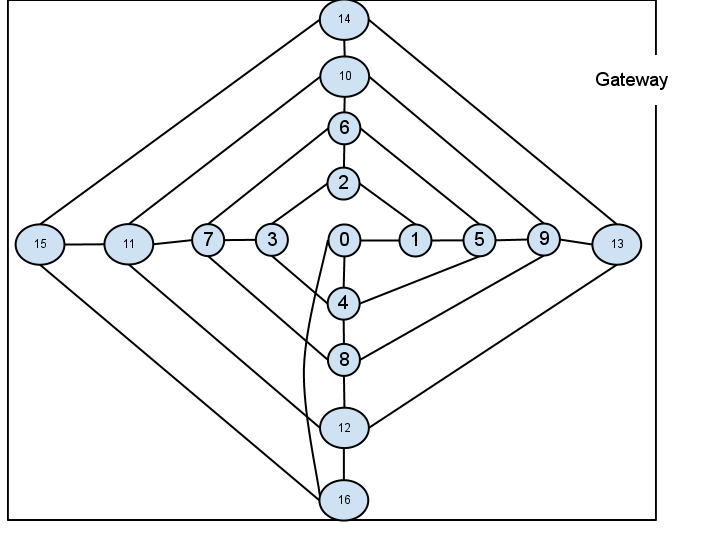
\includegraphics[width=0.5\textwidth]{362prez}
\caption{PBJ Network of Ultra Peers}
\end{figure}
For PBJ, an algorithm for building the network was conceived that attempts to keep all of the nodes in a network within a few hops of each other.  The basic algorithm for connecting ultra nodes in the network can be visualized as an outward spiral of ultra peers, as shown in Figure 1.  While this alone would be wildly inefficient in terms of searching and stability, new ultra nodes also connect to ultra nodes deeper within the spiral.  This allows search requests to quickly move between otherwise distant ultra nodes. More specifically, the first ultra node created will be given an ID of 0, the second an ID of 1, etc.  When an ultra node is created with ID Y, it will attempt to connect to all nodes $X, 0 < X < Y$, where $\log_2 (|Y - X|) = Z , Z$ being an even integer.  So for example, node 16 would connect with node 15 $(16 - 15 = 1 = 2^0)$, node 12 $(16 - 12 = 4 = 2^2)$, and node 0 $(16 - 0 = 16 = 2^4)$.  
A clear benefit of this structure is that the PBJ network has a high level of redundancy in the connections.  This means that the nodes are connected in such a way that it is easy for search requests to reach most, if not all, of the nodes on the network in a few hops.  Currently, the process of actually adding ultra peers to the network and telling them which other ultra peers to connect to is handled through the gateway. The main job of the gateway is to make decisions about how to add a new user node to the network. The gateway keeps track of the status of all the ultrapeers currently in the system.  When a new node tries to join the system, the gateway makes several decisions based on the current status of the PBJ network.  First, the gateway decides if the new node will become an ultra node.  If so, it will give the new ultra node a list of other ultra nodes to connect to.  If the new node is not an ultra node, the gateway will provide information on the appropriate ultra node sub network to join. These decisions by the gateway essentially dictate how the network is built.  As implemented, the first node to enter the network becomes ultra node 0.  If, for example, there are three nodes per ultra node, the next three nodes to connect would become node 0`s sub network.  The fifth node to join the network would become ultra node 1 and would connect to ultra node 0. In this scheme of building the network, each ultra node`s sub network is filled before the next ultra node is created.  This algorithm ensures that the graph has the smallest number of ultra nodes possible in a system since all existing ultra node sub networks must be filled before a new ultra node is created.


\subsection{Searching the Network}


The PBJ client allows the user to share the contents of a directory. The default share directory is a sub-directory named `Share`. All files and sub directories in the user`s share directory will be available to the network for other nodes to download. As figure 2 shows, when a user wants to search for a file, they enter a keyword and submit a search request.  The search request will be sent to the searching node`s ultra node (unless the node is itself an ultra node).
\begin{figure}[tbh]
\centering

\includegraphics[width=0.5\textwidth]{search}
\caption{Searching For a File}
\end{figure}


 The ultra node will send the search request to all of the other peers in its sub network while simultaneously broadcasting it to its connected ultra peers.  Search requests consist of four major parts - the searching node`s address, the keyword, a search id, and the time to live (ttl).  The ttl is initially set to a positive integer.  Each time a search request is passed between ultra peers, the request ttl is decremented.  Notice that ttl only limits the number of hops among ultra peers, passing a request within an ultra node and its sub network has no effect.  If an ultra node receives a search request with a ttl of 0, it will send the request to its sub network and delete the request.  If the keyword is found in any part of a filename, the finding node sends a message to the search node with its IP address and the path of the desired file relative to the share folder.  As these acknowledgement messages come into the search node, it displays to the user a list of all the files found on the network.  The user can then choose one or more of the files to download.  The searching node directly connects to the node with the selected file and downloads it. 
 
 The search ID was added as part of the search request as an attempt to significantly lessen the search request traffic on the network.  The structure of the PBJ network means there are many different paths between any two ultra nodes.  While this is very useful in keeping the network stable and allowing search requests to quickly reach a large number of files, it also means that the same ultra node will receive and process a request multiple times, sending the message out to all of its ultra peers, who have already received the request.  This type of network behavior is extremely inefficient.  PBJ attempts to fix this problem in part by having a unique pair of values in each search request.  One of these values is the IP address of the requester and the other is a search ID that is local to each node and represents the number of requests previously sent out by that node. Together, this (address, search ID) pair make a unique request identifier. Each node keeps track of the last several request ID pairs received and if the request ID pair of a newly received search request matches one in the list, that request is ignored.  This scheme vastly cuts down the amount of redundant request traffic and makes the system more efficient as a whole.
     
\subsection{Disconnecting from the Network}
An area of contention during development of PBJ was how to correctly handle ultra peer disconnection.  Various solutions were proposed, including updating the gateway, electing a node from the sub network to be a new ultra node, and the Ostrich approach (ignoring it).  We eventually decided to implement a heartbeat system, where the gateway checks on existing ultra nodes.  Upon receiving a request to add a new node to the network, the gateway pings every ultra node in the network. If one or more does not respond, the gateway marks those as missing, and inserts ultra nodes into these positions until they are all filled. The point here is to ensure that important connections in the network are rebuilt before attempting to refill the sub networks of ultra nodes. In addition, ultra nodes have a �heartbeat�; they occasionally ping their ultra peers and sub network.  If an ultra node does not get a response from an ultra peer, it removes it from the list of connected ultra peers.  If an ultra peer cannot connect to a peer in its sub network, it removes that peer from its list and notifies the gateway that a spot has opened up in its sub network.  If a node in a sub network cannot reach its ultra peer, it re enters the network through the gateway.  This ensures that all lost nodes will be replaced as new ones are added to the system, and that the network will not become fractured with high node turnover.  


\section{Implementation}
PBJ was written and implemented using Python version 2.7. The code written specifically for PBJ totals approximately 1500 lines.
All of the PBJ network communication is facilitated through the use of the Flask python framework. Flask ~\cite{flask} is a web micro-framework that is designed to simplify the development of Python web applications. HTTP was chosen as a protocol over TCP due to its reliability, simplicity, and flexibility. Flask trivializes the implementation of custom HTTP responses. Every node, as well as the gateway, is running an instance of a Flask server. The instance of the Flask server is told to use a random port that is not currently in use.
To install and use Flask on a machine without modifying any system files, PBJ uses virtualenv ~\cite{virtual}, which is a tool used to create virtual Python environments. A virtual Python environment can be created in a users home folder on a system using virtualenv, and then that user has permission to modify that environment however they wish. In this way, we were able to deploy a Python environment with the Flask module and its dependencies installed on every machine running PBJ.
A concern when laying out the specification of how nodes would communicate was the case in which a node would have to communicate across a firewall. Firewalls add a great deal of complexity when designing a distributed system that is intended to be accessed by a large number of computers under diverse network constraints. Since PBJ is currently academic in nature and limited in resources, we chose to ignore the cases in which communication over the allocated port is unavailable to a node.



\section{Results}
\subsection{Test Plan}
In the design phase of our project, we thoroughly discussed the use of Condor ~\cite{condor}, a HTC application that can deploy processes to a large number of computers, to test our network stability and search algorithms for large numbers of nodes. Unfortunately, the computers on Clemson`s Condor network are equipped with Windows Firewall, which blocks the access of ports that have not been explicitly granted permission. Instead, we ran tests on Clemson`s Palmetto cluster, a 12,000 core Linux cluster ~\cite{palmetto}. Our account on the cluster utilized a shared network drive between nodes, so we had to write a script that would create a unique share file in a unique share directory for every single node. Each node was to have a single shared file to keep search results to a minimum for testing purposes. The end result was a test environment in which 300 searchable nodes with unique files were connected to our network.  As our results demonstrate, the performance of PBJ depends on the total number of ultra nodes in the system. Performance is dramatically affected when the total number of ultra nodes reaches an even power of 2. We were unable to obtain more than 1024 nodes from Palmetto. This lead us to choose 300 test nodes because it was sufficiently above 256.     


We chose to focus our testing on search performance and the scalability of our network structure. To test this, we first eliminated the sub networks so that every new node was designated as an ultra node. We then added additional functionality to the nodes to allow the gateway to tell a node to initiate a search. We designated ultra node 0 to be the searching node for our testing cases. The gateway was modified so that it initiated a wildcard search from node 0 upon the addition of a new node to the network. Node 0 was to log the time the search took for each result, as well as how many hops the request made until each result was found. Nodes were added to the network at intervals of one second, which resulted in 300 discrete test results that describe the scalability of our system. 

\begin{figure}[tbh]
\centering
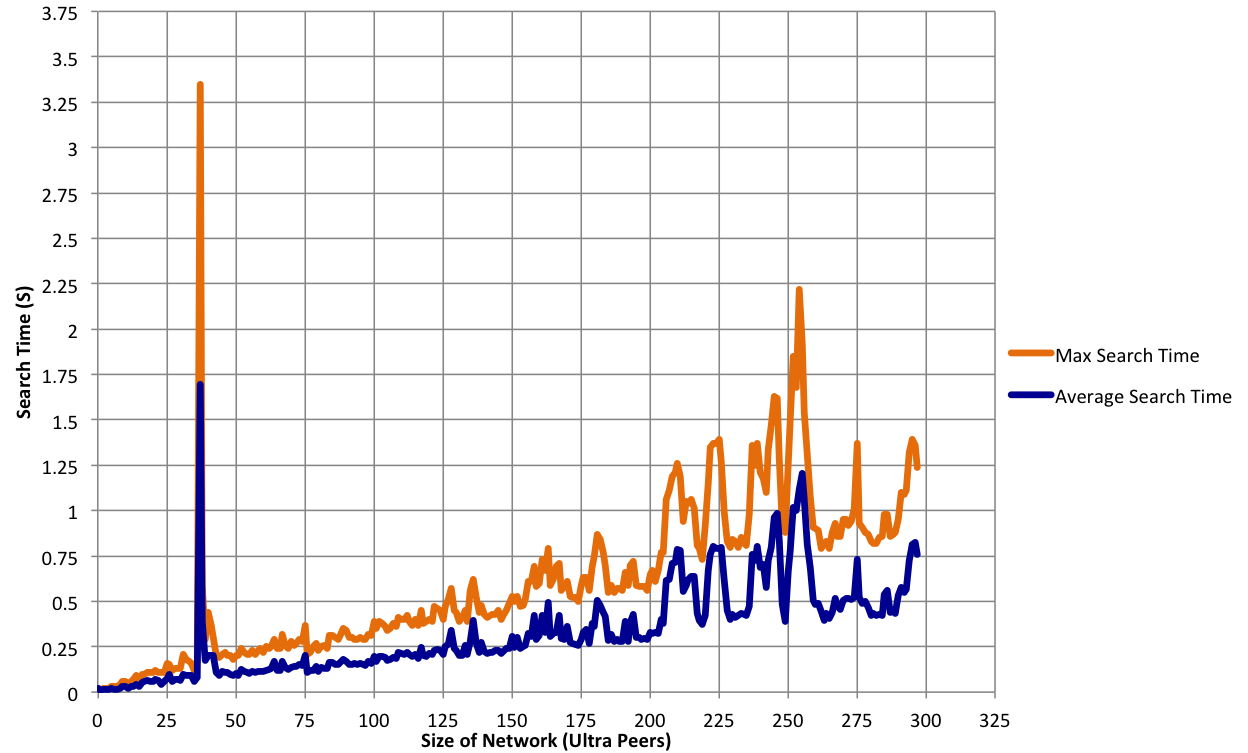
\includegraphics[width=0.5\textwidth]{searchTime}
\caption{Search Time to Reach All Nodes in a Network}
\end{figure}




\subsection{Analysis}

Figure 3 shows the search time results show a positive linear trend with some obvious noise distortion.  Many of the spikes in search time are likely due to network latency.  When ultra node 0 reaches its next connection with ultra node 256, both the average and total search time become much less volatile, likely due to the fact that far fewer hops are now required to reach the highest ultra peers. These numbers represent an idle network where the only messages being passed are search requests from ultra node 0.
In actual use, there would be many messages concurrently, so it is likely that search times would be higher than shown here. Since the majority of this time depends on the latency of the network and the ability of ultra peers to handle large numbers of search requests, an ideal configuration would have the users with the strongest network connections serve as ultra peers.  Several studies have shown that taking advantage of the underlying structure of the physical network can lead to better search times in gnutella ~\cite{Ripeanu}.  A similar approach here would be beneficial.       


\begin{figure}[tbh]
\centering
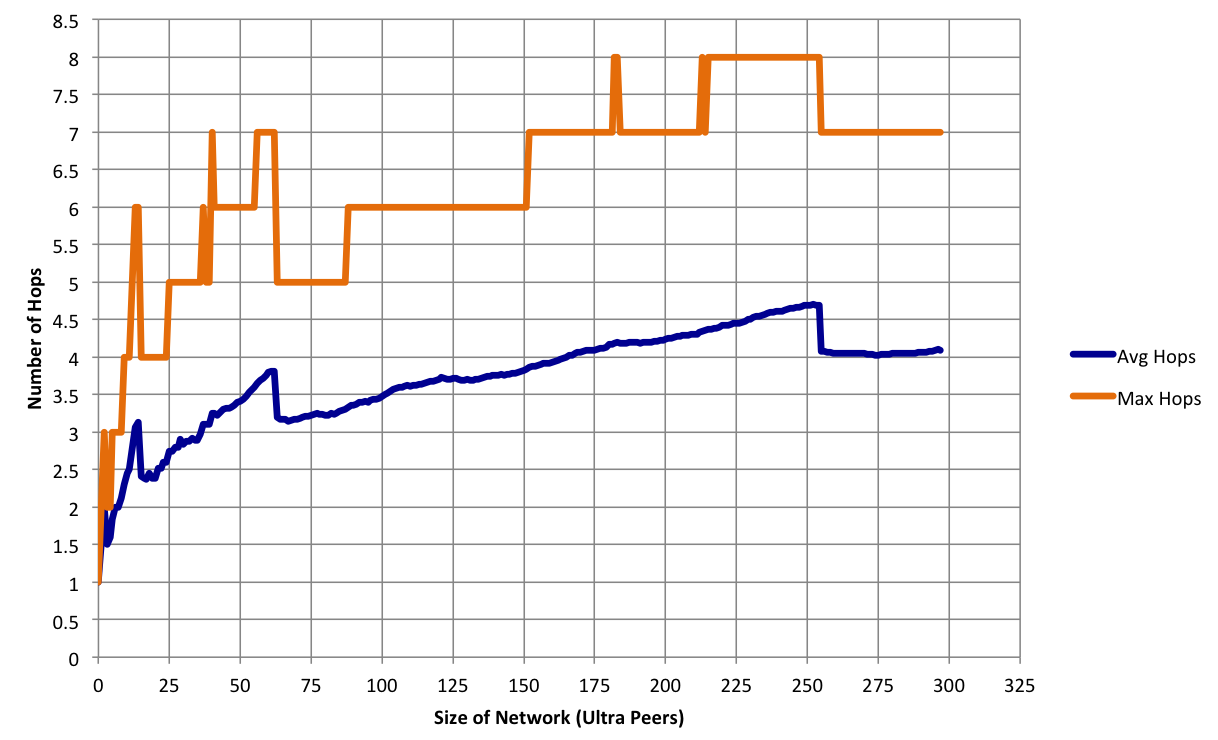
\includegraphics[width=0.5\textwidth]{hops}
\caption{Number of Hops to Reach All Nodes in a Network}
\end{figure}


Figure 4 demonstrates a high correlation between network structure and the number of hops required to reach all the nodes on the system.  Looking at the average number of hops to reach every ultra peer in a network, several trends become apparent.  First, every time an ultra peer with an even power of two connects to ultra peer 0, (ultra peers 4, 16, 64, and 256) the average number of hops to traverse the network decreases, usually by approximately half a hop. This drop occurs because ultra node 0 now has an additional connection through which it can reach other nodes.  Also, this new connection will facilitate sending requests to nodes that were previously farthest away from node 0. This explains why the drop in  the average number of hops is so large when a new connection is added.  Once this drop has occurred, as new ultra peers are added to the network, the average number of hops grows at a roughly linear rate to about one more hop on average than the previous peak.  Notice that the slope of a trend line drawn between a trough and next peak decreases with an increasing number of nodes. This implies that as PBJ gets more and more ultra peers, the addition of ultra peers will have less of an impact on average number of hops to find a file. As the network grows, so does the level of redundancy in the network. More potential pathways between two ultra peers are created and the loss of ultra peers will have less of an effect on the functionality of the whole system.  Since PBJ replaces holes in the network of ultra peers before expanding the network, PBJ is relatively successful at ensuring that redundancy is not lost with the constant logging in and out of users.     


The data for the maximum number of hops to traverse the network seems to imply that a pre-defined ttl would quickly limit the ability of the network to find files in the system.  Initially, the maximum number of hops is very unstable, with large changes between a few ultra peers.  As ultra peers are added to the network the maximum number of hops needed to reach a node in the network seems to fall into a step function, with long stretches of no change.   

Our testing demonstrated to us the stability of the network. To a large extent, the main goals of the project were met. A network of connected peers could be created using only a slightly centralized bootstrapping process, while keeping file searching and downloading completely decentralized. We discovered that there was a large amount of traffic on the network between the pinging of peers and redundant searching, even reduced as it is with the unique request ID. We also feel that an explicit ttl will eventually limit PBJ`s scalability. Based on this testing, we have a number of future improvements to PBJ.  These improvements would increase the network`s stability, decrease redundant traffic, and reach a larger percentage of the network.






\section{Conclusions and Future Work}

PBJ is a decentralized file sharing system network building and search algorithms and node loss handling form the basis for a stable and reliable P2P application. PBJ users connect to the system through a dedicated gateway, either becoming ultra nodes connected to other ultra nodes or part of an ultra node`s sub network. To ensure the refilling of holes in the network, the gateway and the nodes have a �heartbeat�. The gateway maintains the structure of the network and will fill in missing ultra nodes to facilitate reliability and efficiency. Searching the network is done by keyword comparison to filenames, and search requests are broadcast between ultra peers. Results are reported to the searching node, which then has the option of downloading the file from any of the responding nodes.

We tested the scalability of our network using Clemson Unversity`s Palmetto cluster, which allowed us to fill our network with 300 ultra nodes. To test the scalability of our network, we ran an automated test that measured the speed and distance traveled by a search request as the network grew in size. What we found is that even with 300 ultra nodes, the maximum number of hops that a search request took was only 8. Because there is no limit to the number of nodes in an ultra node`s sub network, this shows our network is able propagate a request to an extremely large number of nodes with a minimal number of hops.

In the future, we would like to pursue several possible improvements to PBJ.  One improvement which has been discussed is decentralizing the bootstrapping process by decentralizing the gateway. As our results show, the network�s performance improves once the total number of ultra nodes reaches an even power of 2. An algorithm that takes advantage of this trait would slightly alter how the network is built by the gateway. The basic idea would be to create an ultra peer back bone with empty sub networks and then fill in the sub networks. Another potential improvement would be to choose ultra peers based on network quality. Ultra peers have to handle the vast majority of the network traffic. It then makes sense that the machines with the strongest network connection should be ultra peers. This would help stabilize the network and improve quality. Improvements could also be made to PBJ�s search algorithm, specifically its handling of search ttl. It may make sense to have a ttl that scales with the size of the network, or to remove ttl altogether from searching. Simple things such as an improved GUI and security/privacy features could also be added to make the system more user friendly. Another concern we have is attempting to mitigate is leeching, the practice where by users of a file sharing network do not share any files to be downloaded but still use the network to get files.



% conference papers do not normally have an appendix




% use section* for acknowledgement

% trigger a \newpage just before the given reference
% number - used to balance the columns on the last page
% adjust value as needed - may need to be readjusted if
% the document is modified later
%\IEEEtriggeratref{8}
% The "triggered" command can be changed if desired:
%\IEEEtriggercmd{\enlargethispage{-5in}}


% references section


% can use a bibliography generated by BibTeX as a .bbl file
% BibTeX documentation can be easily obtained at:
% http://www.ctan.org/tex-archive/biblio/bibtex/contrib/doc/
% The IEEEtran BibTeX style support page is at:
% http://www.michaelshell.org/tex/ieeetran/bibtex/
%\bibliographystyle{IEEEtran}
% argument is your BibTeX string definitions and bibliography database(s)
%\bibliography{IEEEabrv,../bib/paper}
%
% <OR> manually copy in the resultant .bbl file
% set second argument of \begin to the number of references
% (used to reserve space for the reference number labels box)
\begin{thebibliography}{99}


\bibitem{evo}
Amir H. Rasti, Daniel Stutzach, Reza Rejaie, "On the Long term Evolution of the Two Tier Gnutella Overlay", in \emph{INFOCOM Proceedings}, Barcelona, Spain, 2006, pp 1 - 6
\bibitem{napster}
Napster Website: http://www.napster.com
\bibitem{bit}
BitTorrent Website: http://www.bittorrent.com/
\bibitem{compare}
Dimitrios Tsoumakos and Nick Roussopoulos. (2011, 11, 20) "A comparison of Peer to Peer Search Methods" [Online]. Available : Google Scholar
\bibitem{flask}
Flask Website : http://flask.pocoo.org/
\bibitem{virtual}
Virtualenv Website : http://www.virtualenv.org/en/latest/index.html
\bibitem{lookup}
Hari Balakrishnan et al, "Looking Up Data in P2P Systems". \emph{Communications of the ACM}, vol 46, No 3,  February, 2003.
\bibitem{study}
Hendrik Schuleze and Klaus Mochalski. "Internet Study 2008/2009". Ipoque Leipzig Germany, 2009
\bibitem{nap}
Original Napster Specification : http://opennap.sourceforge.net/napster.txt
\bibitem{superpeer}
Alper Tugay Misrak et al. "Structured Superpeers: Leveraging Heterogeneity to Provide Constant-Time Lookup" . \emph{WIAPP 2003 Proceedings}
\bibitem{gnut}
Gnutella Website : rfc-gnutella.sourceforge.net
\bibitem{saroiu}
S. Saroiu, P. Gummadi, S. D. Gribble,  \emph{A Measurement Study of Peer-to-Peer File Sharing Systems}, 
University of Washington Technical Report UW-CSE-01-06-02, July 2001.
\bibitem{adar}
Eytan Adar , Bernardo A. Huberman. " Free Riding on Gnutella". 2000
\bibitem{Ripeanu}
Matei Ripeanu, Adriana Iamnitchi, Ian Foster. "Mapping the Gnutella Network". \emph{IEEE Internet Computing}, January-February 2002.  
\bibitem{condor}
Condor Website : http://research.cs.wisc.edu/condor/
\bibitem{palmetto}
Palmetto Cluster Website : citi.clemson.edu/palmetto

\end{thebibliography}








% that`s all folks
\end{document}



